\chapter{Appendix}
\section{Calculations}
\subsection{Creation and Annihilation Operators}
The creation and annihilation operators in k-space can be defined as follows (symmetric normalization factors, and the number of unit cells in the chain $N_d = \nicefrac{N}{2}$):
\begin{align}
c_{2n} &= \frac{1}{\sqrt{N_d}}\sum_k\exp\left[ik\left(2n\right)a\right]\cdot c_{k}^{(e)}\\
c_{2n+1} &= \frac{1}{\sqrt{N_d}}\sum_k\exp\left[ik\left(2n+1\right)a\right]\cdot c_{k}^{(o)}\\
c_k^{(e)} &= \frac{1}{\sqrt{N_d}}\sum_n \exp\left[-ik\left(2n\right)a\right]\cdot c_{2n}\\
c_k^{(o)} &= \frac{1}{\sqrt{N_d}}\sum_n \exp\left[-ik\left(2n+1\right)a\right]\cdot c_{2n+1}
\end{align}
Exemplary check for self-consistency:
\begin{align}
c_{2n_0}\left(c_k^{(e)}(c_{2n})\right) &= \frac{1}{\sqrt{N_d}}\sum_k\exp\left[ik\left(2n_0\right)a\right]\cdot \frac{1}{\sqrt{N_d}}\sum_n \exp\left[-ik\left(2n\right)a\right]\cdot c_{2n}\\
&= \frac{1}{N_d}\sum_{k, n} \exp\left[ika\left(2n_0-2n\right)\right]\cdot c_{2n}\\
&= \frac{1}{N_d}\sum_n N_d\cdot \delta_{2n_0,2n}\cdot c_{2n}\\
&= c_{2n_0}
\end{align}
Auxiliary calculations for later:
\begin{align}
\sum_n^{N_d}c_{2n+1}^\dagger c_{2n} &=\sum_{n, k, k'} \exp\left[ika(2n)\right] \cdot \exp\left[-ik'a(2n+1)\right] \cdot \frac{c_{k'}^{\dagger(o)}c_k^{(e)}}{N_d} \\
&=\sum_{n, k, k'} \exp\left[ia(k-k')(2n)\right] \cdot \exp\left(-ik'a\right) \cdot  \frac{c_{k'}^{\dagger(o)}c_k^{(e)}}{N_d} \\
&=\sum_{k, k'} \delta_{k, k'} \cdot \exp\left(-ik'a\right)\cdot c_{k'}^{\dagger(o)}c_k^{(e)}\\
&=\sum_{k'} \exp\left(-ik'a\right) \cdot c_{k'}^{\dagger(o)}c_{k'}^{(e)}
\end{align}
Analogously:
\begin{align}
\sum_n^{N_d} c_{2n}^\dagger c_{2n+1} &=\sum_{k'} \exp\left(ik'a\right)\cdot c_{k'}^{\dagger(e)}c_{k'}^{(o)}\\
\sum_n^{N_d} c_{2n}^\dagger c_{2n-1}&=\sum_{k'} \exp\left(-ik'a\right)\cdot  c_{k'}^{\dagger(e)}c_{k'}^{(o)}\\
\sum_n^{N_d} c_{2n-1}^\dagger c_{2n} &=\sum_{k'} \exp\left(ik'a\right)\cdot  c_{k'}^{\dagger(o)}c_{k'}^{(e)}
\end{align}
\subsection{Transformation of the SSH-Hamiltonian}
Using the relations of the previous section the Hamiltonian from \cref{equation_SSH_hamiltonian_real_space} can be transformed as follows:
\begin{align}
\mathcal{H} &= -2\sum_n^{N_d} \left[\left(t_0+\delta\right)\left(c_{2n+1}^\dagger c_{2n} + c_{2n}^\dagger c_{2n+1} \right) + 
\left(t_0-\delta\right)\left(c_{2n+2}^\dagger c_{2n+1} + c_{2n+1}^\dagger c_{2n+2}\right)\right]+2N\kappa u^2\\
&= -2\sum_{k'} \left[\left(t_0+\delta\right)\left(\exp\left(-ik'a\right) \cdot c_{k'}^{\dagger(o)}c_{k'}^{(e)} + \exp\left(ik'a\right)\cdot c_{k'}^{\dagger(e)}c_{k'}^{(o)}\right)+ \right.\nonumber\\
&\hspace*{1.6cm}\left.\left(t_0-\delta\right)\left(\exp\left(-ik'a\right)\cdot  c_{k'}^{\dagger(e)}c_{k'}^{(o)}+\exp\left(ik'a\right)\cdot  c_{k'}^{\dagger(o)}c_{k'}^{(e)}\right)\right]+2N\kappa u^2\\
&= -2\sum_{k'} \left\{\left[2t_0\cos(k'a) + 2i\delta\sin(k'a)\right]c_{k'}^{\dagger(e)}c_{k'}^{(o)} + \right.\nonumber\\
&\hspace*{1.7cm}\left. \left[2t_0\cos(k'a)-2i\delta\sin(k'a)\right] c_{k'}^{\dagger(o)}c_{k'}^{(e)}\right\}+2N\kappa u^2
\end{align}
Substituting $\epsilon_k := 2t_0\cos(ka)$ and $\Delta_k := 2\delta\sin(ka)$ the following form of the hopping term can be derived:
\begin{align}
\mathcal{H}_{\text{hopp},k} &=
\left[\epsilon_k + i\Delta_k\right]c_{k}^{\dagger(e)}c_{k}^{(o)} + \left[\epsilon_k-i\Delta_k \right]	c_{k}^{\dagger(o)}c_{k}^{(e)}
\end{align}
\subsection{Calculation of the Average HOMO-Band Energy}
The average energy of the hopping term for the HOMO-band can be calculated as follows:
\begin{align}
E_A &=-\frac{1}{N_d}\sum_k |E_k|\\
&= -\frac{1}{N_d}\sum_k \sqrt{\left[2t_0\cos(ka)\right]^2+\left[2\delta\sin(ka)\right]^2}
\end{align}
In the limit of $N_d \rightarrow \infty$ (infinite chain) the sum becomes an integral:
\begin{align}
E_A &= -\frac{1}{\pi}\int\limits_{\nicefrac{-\pi}{2}}^{\nicefrac{\pi}{2}}\hspace*{-0.2cm}\text{d}\theta\ \sqrt{\left[2t_0\cos(\theta)\right]^2+\left[2\delta\sin(\theta)\right]^2}\\
&=-\frac{4t_0}{\pi}\underbrace{\int\limits_{0}^{\nicefrac{\pi}{2}}\text{d}\theta\ \sqrt{1-\left(1-\frac{\delta^2}{t_0^2}\right)\sin^2(\theta)}}_{=:F(\nicefrac{\delta}{t_0})}
\end{align}
with the complete elliptical integral of the second kind $F(x)$. Later $F(x) \approx 1$ for $|x|\ll 1$ is used.

\subsection{Calculation of the Ground State Energy for the First Method}
The expectation value of the hopping energy can be calculated as follows:
\begin{align}
\left\langle\Psi_k^{(v)}(q)\Big|\mathcal{H}_{\text{hopp},k}\Big|\Psi_k^{(v)}(q)\right\rangle &= \left[\sqrt{\frac{1-q}{2}}c_k^{(e)}- \sqrt{\frac{1+q}{2}}\frac{\epsilon_k + i \Delta_k}{|E_k|}c_{k}^{(o)}\right]\cdot\nonumber\\
&\hspace*{0.5cm}\left[
\left[\epsilon_k + i\Delta_k\right]c_{k}^{\dagger(e)}c_{k}^{(o)} + \left[\epsilon_k-i\Delta_k \right]	c_{k}^{\dagger(o)}c_{k}^{(e)}
\right]\cdot\nonumber\\
&\hspace*{0.5cm}\left[\sqrt{\frac{1-q}{2}}c_k^{\dagger(e)}- \sqrt{\frac{1+q}{2}}\frac{\epsilon_k - i \Delta_k}{|E_k|}c_{k}^{\dagger(o)}\right]\\
&=-\sqrt{\frac{1-q}{2}}c_k^{(e)}\left[\epsilon_k+i\Delta_k \right]	c_{k}^{\dagger(e)}c_{k}^{(o)}\sqrt{\frac{1+q}{2}}\frac{\epsilon_k - i \Delta_k}{|E_k|}c_{k}^{\dagger(o)}\nonumber\\
&\hspace*{0.4cm}-\sqrt{\frac{1+q}{2}}\frac{\epsilon_k + i \Delta_k}{|E_k|}c_{k}^{(o)}\left[\epsilon_k - i\Delta_k\right]c_{k}^{\dagger(o)}c_{k}^{(e)}\sqrt{\frac{1-q}{2}}c_k^{\dagger(e)}\\
&=-\sqrt{\frac{1+q}{2}}\sqrt{\frac{1-q}{2}}\left[\frac{(\epsilon_k-i\Delta_k)(\epsilon_k+i\Delta_k)}{|E_k|}+\frac{(\epsilon_k-i\Delta_k)(\epsilon_k+i\Delta_k)}{|E_k|}\right]\\
&= -\sqrt{1-q^2} |E_k|
\end{align}
Thus the sum over the HOMO-band hopping energies becomes for small $\nicefrac{\delta}{t_0}$:
\begin{align}
E_0(q) &= -\frac{4Nt_0}{\pi} \sqrt{1-q^2}
\end{align}
\subsection{Calculation of the Average HOMO-Band Energy for the Second Method}
Then the HOMO-band energy sum can be calculated as follows:
\begin{align}
E_A &= -\frac{1}{N_d}\sum_k |E_k|\\
&= -\frac{1}{N_d}\sum_k \sqrt{V^2 + 4t_0^2\cos^2(ka) + 4 \delta^2\sin^2(ka)}\\
&= -\frac{1}{N_d}\sqrt{V^2 + 4t_0^2}\sum_k \sqrt{1 - c^2 \cdot \sin^2(ka)}
\end{align} 
with $c^2 = \frac{4t_0^2-4\delta^2}{V^2+4t_0^2}$. In the limit of $N \to \infty$ (number of $k$-points is $N_d = \nicefrac{N}{2}$) the sum can be transformed into an integral:
\begin{align}
E_A &= -\frac{2}{\pi} \sqrt{V^2+4t_0^2} \int\limits_{0}^{\nicefrac{\pi}{2}} \text{d}\theta \sqrt{1 - c^2 \cdot \sin^2(\theta)}\\
&= -\frac{2}{\pi} \sqrt{V^2+4t_0^2} \cdot F(\sqrt{1-c^2}) 
\end{align}

\section{Convergence Testing of the Hydrogen Chain}

\begin{figure}[!h]
	\centering
	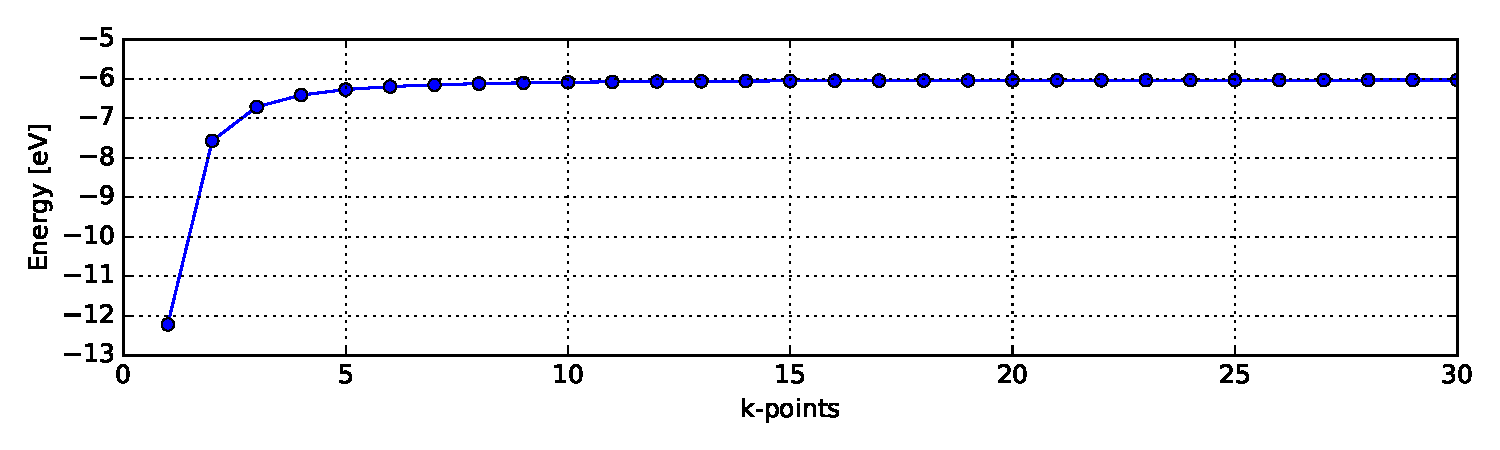
\includegraphics[width = 13cm]{Images/Hydrogen/convergence/kpts-energy}
	\caption{Ground state energy of the hydrogen chain (unit cell containing two hydrogen atoms) in respect to the number of $k$-points.}
	\label{}
\end{figure}
\begin{figure}[!h]
	\centering
	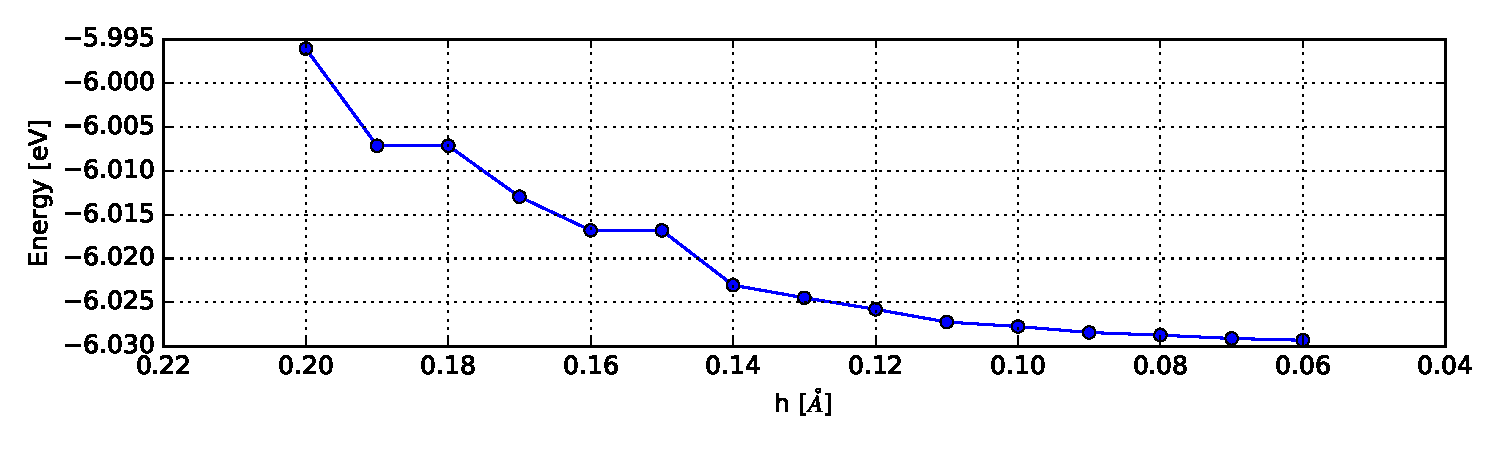
\includegraphics[width = 13cm]{Images/Hydrogen/convergence/gridspacing-energy}
	\caption{Ground state energy of the hydrogen chain (unit cell containing two hydrogen atoms) in respect to the grid spacing $h$.}
	\label{}
\end{figure}
\begin{figure}[!h]
	\centering
	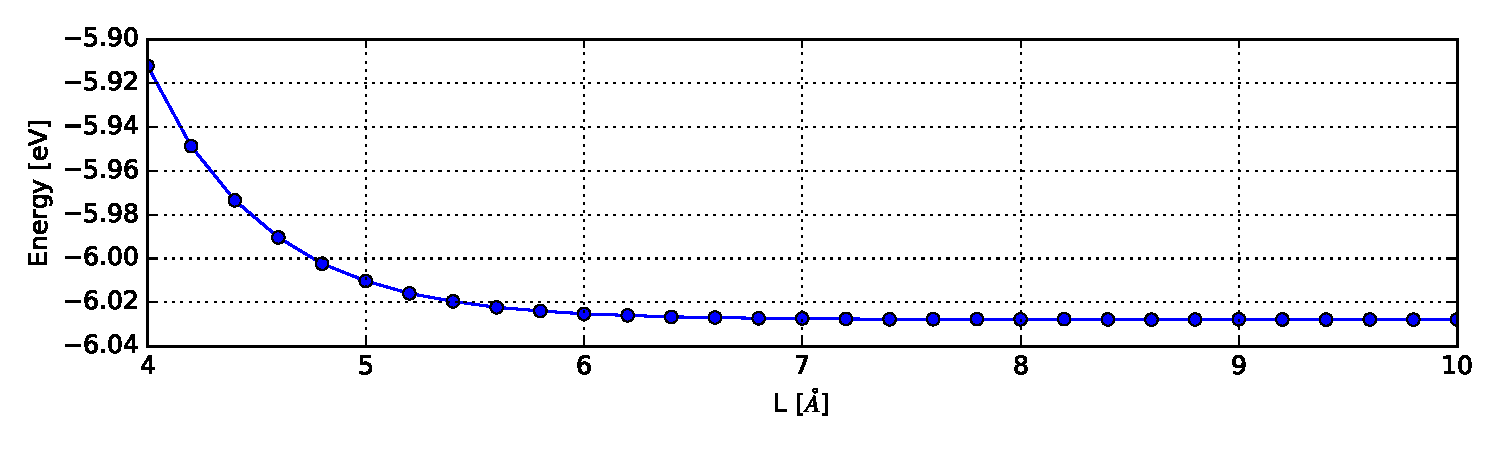
\includegraphics[width = 13cm]{Images/Hydrogen/convergence/unit_cell_width}
	\caption{Ground state energy of the hydrogen chain (unit cell containing two hydrogen atoms) in respect to the cell width $L$ (not in direction of periodic boundary condition).}
	\label{}
\end{figure}

